% !TEX root = task-3-21-2.tex
% Editable task bank. Append new BankTask blocks at the end of the document.
\documentclass[12pt,a4paper]{article}
\usepackage{physics-textbook}
\usepackage{graphicx,needspace}
\usetikzlibrary{decorations.pathmorphing}
\newif\ifShowSolutions
\ifdefined\TutorEdition
  \ShowSolutionstrue
\else
  \ShowSolutionsfalse % Change to \ShowSolutionstrue to display solutions.
\fi
\newcounter{banktask}
\newsavebox{\BankTaskBox}
\newcommand{\BankTaskContent}[3]{%
  \noindent\textbf{\thebanktask.}\quad #2\par
  \ifShowSolutions
    \Needspace{50mm}% Keep the solution heading with its opening text or diagram.
    #3\par
    \ifdefined\TutorEdition
      \ifcsname TutorSource#1\endcsname
        \nopagebreak\smallskip{\small\csname TutorSource#1\endcsname\par}%
      \fi
    \fi
  \fi
}
\newcommand{\BankTask}[3]{%
  \refstepcounter{banktask}\par\medskip
  \sbox{\BankTaskBox}{\begin{minipage}{\linewidth}%
    \BankTaskContent{#1}{#2}{#3}\end{minipage}}%
  \ifdim\dimexpr\ht\BankTaskBox+\dp\BankTaskBox\relax>\dimexpr\textheight-20mm\relax
    \Needspace{35mm}\BankTaskContent{#1}{#2}{#3}%
  \else
    \Needspace{\dimexpr\ht\BankTaskBox+\dp\BankTaskBox\relax}%
    \noindent\usebox{\BankTaskBox}\par
  \fi
  \medskip
}
\begin{document}
\BookSubsection{3.21.2}{Энергетические превращения в колебательном контуре}


% Source CFDDFB: https://ege.fipi.ru/bank/questions.php?search=1&proj=BA1F39653304A5B041B656915DC36B38&qid=CFDDFB
\BankTask{CFDDFB}{
Конденсатор, заряженный до разности потенциалов $U$, в первый раз подключили к катушке с индуктивностью $L$, а во второй — к катушке с индуктивностью $4L$. Каково отношение периодов колебаний энергии конденсатора $\dfrac{T_2}{T_1}$ в этих двух случаях? Потерями энергии в контуре пренебречь.
}{
\smallskip\noindent\textbf{Решение от GPT}\par
Энергия конденсатора $W_C=\dfrac{CU^2}{2}\cos^2\omega t$ меняется с периодом $T_W=\dfrac{\pi}{\omega}=\pi\sqrt{LC}$. Следовательно,
\[
\frac{T_2}{T_1}=\sqrt{\frac{4L}{L}}=2.
\]
Ответ: $2$.
}

% Source 91A3F0: https://ege.fipi.ru/bank/questions.php?search=1&proj=BA1F39653304A5B041B656915DC36B38&qid=91A3F0
\BankTask{91A3F0}{
Конденсатор, заряженный до разности потенциалов $U$, в первый раз подключили к катушке с индуктивностью $L_1=L$, а во второй — к катушке с индуктивностью $L_2=4L$. В обоих случаях в получившемся контуре возникли незатухающие электромагнитные колебания. Каково отношение значений полной энергии колебаний $\dfrac{W_2}{W_1}$?
}{
\smallskip\noindent\textbf{Решение от GPT}\par
Полная энергия контура сохраняется и равна начальной энергии заряженного конденсатора: $W=\dfrac{CU^2}{2}$. В обоих случаях ёмкость и начальное напряжение одинаковы, поэтому
\[
\frac{W_2}{W_1}=1.
\]
Ответ: $1$.
}

% Source 93A417: https://ege.fipi.ru/bank/questions.php?search=1&proj=BA1F39653304A5B041B656915DC36B38&qid=93A417
\BankTask{93A417}{
Конденсатор, заряженный до напряжения \(U_0\), в первый раз подключили к катушке с индуктивностью \(L\), а во второй --- к катушке с индуктивностью \(4L\). В обоих случаях в контуре возникли свободные незатухающие электромагнитные колебания. Каково отношение амплитуд силы тока \(\dfrac{I_{2\max}}{I_{1\max}}\) при этих колебаниях?
}{
\smallskip\noindent\textbf{Решение от GPT}\par
По закону сохранения энергии
\[
\frac{CU_0^2}{2}=\frac{LI_{\max}^2}{2},\qquad I_{\max}=U_0\sqrt{\frac{C}{L}}.
\]
Следовательно, \(\dfrac{I_{2\max}}{I_{1\max}}=\sqrt{\dfrac{L}{4L}}=\dfrac12\).
Ответ: \(0{,}5\).
}

% Source 7CCC09: https://ege.fipi.ru/bank/questions.php?search=1&proj=BA1F39653304A5B041B656915DC36B38&qid=7CCC09
\BankTask{7CCC09}{
На рисунке приведён график зависимости силы тока от времени в колебательном контуре. Сколько раз в течение первых $6\text{ мкс}$ энергия конденсатора достигает минимального значения?
\begin{center}
\begin{tikzpicture}[x=0.85cm,y=0.42cm,>=stealth]
\draw[->] (-1,0)--(7.2,0) node[below] {$t,\text{ мкс}$};
\draw[->] (0,-7)--(0,7) node[left] {$I,\text{ мА}$};
\node[below left] at (0,0) {$0$};
\draw (-0.15,5)--(0.15,5) node[left=5pt] {$5$};
\draw (-0.15,-5)--(0.15,-5) node[left=5pt] {$-5$};
\foreach \x in {1,2,3,4,5,6} \draw (\x,0.15)--(\x,-0.15);
\foreach \x in {1,3,5,6} \node[below] at (\x,-0.3) {$\x$};
\draw[thick,smooth,samples=121,domain=0:6] plot (\x,{5*sin(90*\x)});
\end{tikzpicture}
\end{center}
}{
\smallskip\noindent\textbf{Решение от GPT}\par
Энергия конденсатора $W_C=W-\frac{LI^2}{2}$ минимальна при максимальном модуле тока. На графике это моменты $t=1\text{ мкс}$, $3\text{ мкс}$ и $5\text{ мкс}$. Ответ: $3$ раза.
}

% Source Fc855A: https://ege.fipi.ru/bank/questions.php?search=1&proj=BA1F39653304A5B041B656915DC36B38&qid=Fc855A
\BankTask{Fc855A}{
В идеальном колебательном контуре, состоящем из конденсатора и катушки индуктивности, происходят свободные электромагнитные колебания. Изменение заряда конденсатора в колебательном контуре с течением времени показано в таблице.

\begin{center}
\begin{tabular}{|c|c|c|c|c|c|c|c|c|c|c|}
\hline
$t,\ 10^{-6}\,\text{с}$ & $0$ & $1$ & $2$ & $3$ & $4$ & $5$ & $6$ & $7$ & $8$ & $9$ \\
\hline
$q,\ 10^{-9}\,\text{Кл}$ & $1$ & $0{,}71$ & $0$ & $-0{,}71$ & $-1$ & $-0{,}71$ & $0$ & $0{,}71$ & $1$ & $0{,}71$ \\
\hline
\end{tabular}
\end{center}

\begin{enumerate}
\item Период колебаний равен $8\times10^{-6}\,\text{с}$.
\item Частота колебаний равна $250\,\text{кГц}$.
\item В момент времени $t=2\times10^{-6}\,\text{с}$ модуль силы тока в катушке индуктивности максимален.
\item В момент времени $t=8\times10^{-6}\,\text{с}$ энергия магнитного поля катушки индуктивности максимальна.
\item В момент времени $t=4\times10^{-6}\,\text{с}$ энергия электрического поля конденсатора минимальна.
\end{enumerate}
}{
\smallskip\noindent\textbf{Решение от GPT}\par
Заряд возвращается к исходному максимуму через $T=8\times10^{-6}\,\text{с}$, поэтому утверждение 1 верно. Частота $\nu=1/T=125\,\text{кГц}$, поэтому утверждение 2 неверно. При $t=2\times10^{-6}\,\text{с}$ заряд равен нулю, а модуль тока максимален, поэтому утверждение 3 верно. При $t=8\times10^{-6}\,\text{с}$ заряд максимален, ток и энергия магнитного поля равны нулю, поэтому утверждение 4 неверно. При $t=4\times10^{-6}\,\text{с}$ модуль заряда максимален и энергия $W_{\text{эл}}=q^2/(2C)$ максимальна, поэтому утверждение 5 неверно. Ответ: 1, 3.
}

% Source E51107: https://ege.fipi.ru/bank/questions.php?search=1&proj=BA1F39653304A5B041B656915DC36B38&qid=E51107
\BankTask{E51107}{
На рисунке приведён график зависимости силы тока от времени в колебательном контуре, образованном конденсатором и катушкой, индуктивность которой равна $0{,}3\,\text{Гн}$.
\begin{enumerate}
\item Период электромагнитных колебаний в контуре равен $2\,\text{мс}$.
\item Максимальное значение энергии электрического поля конденсатора равно $5{,}4\,\text{мкДж}$.
\item В момент времени $5\,\text{мс}$ заряд конденсатора равен нулю.
\item В момент времени $3\,\text{мс}$ энергия магнитного поля катушки достигает своего минимума.
\item За первые $6\,\text{мс}$ энергия магнитного поля катушки достигла своего максимума $2$ раза.
\end{enumerate}
\begin{center}
\begin{tikzpicture}[book diagram,x=0.62cm,y=0.14cm]
\draw[-{book tip}] (0,-8.4)--(0,10.8);
\draw[-{book tip}] (0,0)--(7.4,0);
\node[above left] at (0,9.3) {$i,\,\text{мА}$};
\node[below right] at (6.65,-0.5) {$t,\,\text{мс}$};
\foreach \x in {1,2,3,4,5,6}{\draw (\x,-0.5)--(\x,0.5);\node[below] at (\x,-0.7) {$\x$};}
\foreach \y in {-6,6}{\draw (-0.12,\y)--(0.12,\y);\node[left] at (-0.18,\y) {$\y$};}
\node[below left] at (-0.08,0) {$0$};
\draw[very thick,smooth,samples=160,domain=0:6] plot (\x,{6*sin(90*\x)});
\end{tikzpicture}
\end{center}
}{
\smallskip\noindent\textbf{Решение от GPT}\par
По графику $T=4\,\text{мс}$, поэтому утверждение 1 неверно. Максимальная энергия электрического поля равна полной энергии контура: $W_{\max}=LI_{\max}^2/2=0{,}3\cdot(6\cdot10^{-3})^2/2=5{,}4\cdot10^{-6}\,\text{Дж}$, поэтому утверждение 2 верно. При $t=5\,\text{мс}$ ток максимален, вся энергия заключена в магнитном поле, а заряд конденсатора равен нулю: утверждение 3 верно. При $t=3\,\text{мс}$ модуль тока максимален, поэтому магнитная энергия максимальна и утверждение 4 неверно. За первые $6\,\text{мс}$ её максимумы достигаются трижды: при $t=1$, $3$ и $5\,\text{мс}$, поэтому утверждение 5 неверно. Ответ: 2, 3.
}

% Source e435F2: https://ege.fipi.ru/bank/questions.php?search=1&proj=BA1F39653304A5B041B656915DC36B38&qid=e435F2
\BankTask{e435F2}{
Идеальный колебательный контур состоит из конденсатора и катушки индуктивности. Напряжение между обкладками конденсатора изменяется во времени в соответствии с формулой \(U(t)=U_m\cdot\cos\omega t\).

Приведённые ниже графики А и Б представляют зависимость физических величин, характеризующих электромагнитные колебания в контуре, от времени \(t\) (\(T\) — период колебаний). Установите соответствие между графиками и физическими величинами, зависимость которых от времени эти графики могут представлять.

\TaskMatchingColumns[.53\linewidth]{Графики}{
А) график А\par
Б) график Б
}{Физические величины}{
1) сила тока в катушке\par
2) энергия магнитного поля катушки\par
3) энергия электрического поля конденсатора\par
4) заряд одной из обкладок конденсатора
}

\medskip
\begin{tabular}{|c|c|}
\hline
А & Б \\
\hline
\phantom{00} & \phantom{00} \\
\hline
\end{tabular}

\medskip
\begin{tikzpicture}[book diagram]
\node at (2.1,1.25) {А)};
\draw[-{book tip}] (0,-1.05)--(0,1.8);
\draw[-{book tip}] (0,0)--(4.55,0) node[below right] {$t$};
\node[below left] at (0,0) {$0$};
\node[below left] at (4,0) {$T$};
\draw plot[domain=0:4.2,samples=101] (\x,{-0.76*sin(90*\x)});
\end{tikzpicture}
\qquad
\begin{tikzpicture}[book diagram]
\node at (2.1,2.55) {Б)};
\draw[-{book tip}] (0,-0.35)--(0,2.5);
\draw[-{book tip}] (0,0)--(4.55,0) node[below right] {$t$};
\node[below left] at (0,0) {$0$};
\node[below] at (4,0) {$T$};
\draw plot[domain=0:4,samples=121] (\x,{2.15*(sin(90*\x))^2});
\end{tikzpicture}
}{
\smallskip\noindent\textbf{Решение от GPT}\par
Заряд \(q=CU_m\cos\omega t\), поэтому сила тока \(I=dq/dt=-\omega CU_m\sin\omega t\): график А соответствует величине 1. Энергия магнитного поля \(W_L=LI^2/2\propto\sin^2\omega t\), поэтому график Б соответствует величине 2. Величины 3 и 4 не подходят: \(W_C=CU_m^2\cos^2\omega t/2\) и \(q=CU_m\cos\omega t\) при \(t=0\) отличны от нуля. Ответ: А — 1, Б — 2.
}

% Source 646A9F: https://ege.fipi.ru/bank/questions.php?search=1&proj=BA1F39653304A5B041B656915DC36B38&qid=646A9F
\BankTask{646A9F}{
На рисунке приведён график зависимости силы тока от времени в катушке индуктивности идеального колебательного контура.

Графики А и Б представляют изменения физических величин, характеризующих колебания в контуре. Установите соответствие между графиками и физическими величинами, зависимость которых от времени эти графики могут представлять.

\TaskMatchingColumns[.53\linewidth]{Графики}{
А) график А\par
Б) график Б
}{Физические величины}{
1) индуктивность катушки\par
2) напряжение на обкладках конденсатора\par
3) энергия электрического поля конденсатора\par
4) энергия магнитного поля катушки
}

\medskip
\begin{tabular}{|c|c|}
\hline
А & Б \\
\hline
\phantom{00} & \phantom{00} \\
\hline
\end{tabular}

\medskip
\begin{tikzpicture}[book diagram]
\draw[-{book tip}] (0,-1.05)--(0,1.8) node[left] {$I$};
\draw[-{book tip}] (-0.18,0)--(3.75,0) node[below right] {$t$};
\node[below left] at (0,0) {$0$};
\draw plot[domain=0:3.3,samples=101] (\x,{0.88*cos(360*\x/3.3)});
\draw[dashed] (3.3,0)--(3.3,0.88);
\node[below] at (3.3,0) {$T$};
\end{tikzpicture}

\medskip
\begin{tikzpicture}[book diagram]
\node at (1.4,1.8) {А)};
\draw[-{book tip}] (0,-0.25)--(0,1.55);
\draw[-{book tip}] (-0.18,0)--(3.12,0) node[below right] {$t$};
\node[below left] at (0,0) {$0$};
\draw plot[domain=0:2.7,samples=121] (\x,{1.15*(cos(360*\x/2.7))^2});
\draw (2.7,0.3)--(2.7,1.15);
\node[below] at (2.7,0) {$T$};
\end{tikzpicture}
\qquad
\begin{tikzpicture}[book diagram]
\node at (1.4,1.8) {Б)};
\draw[-{book tip}] (0,-0.8)--(0,1.3);
\draw[-{book tip}] (-0.18,0)--(3.05,0) node[below right] {$t$};
\node[below left] at (0,0) {$0$};
\draw plot[domain=0:2.78,samples=101] (\x,{0.57*sin(360*\x/2.6)});
\node[below left] at (2.6,0) {$T$};
\end{tikzpicture}
}{
\smallskip\noindent\textbf{Решение от GPT}\par
По исходному графику \(I=I_m\cos\omega t\), поэтому \(W_L=LI_m^2\cos^2\omega t/2\): график А соответствует величине 4. Напряжение \(U=-L\,dI/dt=\omega LI_m\sin\omega t\), что соответствует графику Б и величине 2. Индуктивность (1) постоянна, а энергия электрического поля (3) пропорциональна \(\sin^2\omega t\), неотрицательна и в начальный момент равна нулю, поэтому эти варианты не подходят. Ответ: А — 4, Б — 2.
}

% Source 1FA129: https://ege.fipi.ru/bank/questions.php?search=1&proj=BA1F39653304A5B041B656915DC36B38&qid=1FA129
\BankTask{1FA129}{
Идеальный колебательный контур состоит из конденсатора электроёмкостью \(50\text{ мкФ}\) и катушки индуктивности. Заряд на одной из пластин конденсатора изменяется во времени в соответствии с формулой \(q(t)=4\cdot10^{-4}\cdot\sin(2000t)\) (все величины выражены в СИ).

Установите соответствие между физическими величинами и формулами, выражающими их зависимость от времени в условиях данной задачи.

\TaskMatchingColumns[0.53\linewidth]{Физические величины}{
А) напряжение \(u(t)\) на обкладках конденсатора\par
Б) энергия \(W_C(t)\) электрического поля конденсатора
}{Формулы}{
1) \(1{,}6\cdot10^{-3}\cdot\sin^2(2000t)\)\par
2) \(8\cdot\sin(2000t)\)\par
3) \(1{,}6\cdot10^{-3}\cdot\cos^2(2000t)\)\par
4) \(0{,}8\cdot\sin\left(2000t-\frac{\pi}{2}\right)\)
}

\medskip
\begin{tabular}{|c|c|}
\hline
А & Б \\
\hline
\phantom{00} & \phantom{00} \\
\hline
\end{tabular}
}{
\smallskip\noindent\textbf{Решение от GPT}\par
Напряжение \(u(t)=q(t)/C=8\sin(2000t)\text{ В}\), поэтому А соответствует формуле 2. Энергия \(W_C(t)=q^2(t)/(2C)=1{,}6\cdot10^{-3}\sin^2(2000t)\text{ Дж}\), поэтому Б соответствует формуле 1. Формула 3 имеет неверную начальную фазу энергии, а формула 4 не соответствует ни напряжению по амплитуде и фазе, ни неотрицательной энергии. Ответ: А — 2, Б — 1.
}

% Source D71C20: https://ege.fipi.ru/bank/questions.php?search=1&proj=BA1F39653304A5B041B656915DC36B38&qid=D71C20
\BankTask{D71C20}{
Идеальный колебательный контур состоит из конденсатора и катушки индуктивностью $L$. Напряжение на пластинах конденсатора изменяется во времени в соответствии с формулой $u(t)=U_0\sin\omega t$.

Установите соответствие между физическими величинами и формулами, выражающими их зависимость от времени.

\begin{center}
\TaskMatchingColumns[0.48\linewidth]{Физические величины}{
А) сила тока $i(t)$ в колебательном контуре\par
Б) энергия $W_L(t)$ магнитного поля катушки
}{Формулы}{
1) $\displaystyle\frac{U_0^2}{2L\omega^2}\cos^2\omega t$\par
2) $\displaystyle\frac{U_0}{\omega L}\cos\omega t$\par
3) $\displaystyle\frac{U_0^2}{2L\omega^2}\cdot\sin^2\omega t$\par
4) $\displaystyle\frac{\omega L}{U_0}\sin\omega t$
}

\begin{tabular}{|c|c|}
\hline
А & Б \\
\hline
\phantom{22} & \phantom{22} \\
\hline
\end{tabular}
\end{center}
}{
\smallskip\noindent\textbf{Решение от GPT}\par
Из $\omega^2=1/(LC)$ получаем $C=1/(L\omega^2)$, поэтому $i(t)=C\,du/dt=\dfrac{U_0}{L\omega}\cos\omega t$: А — 2. Энергия магнитного поля $W_L(t)=Li^2/2=\dfrac{U_0^2}{2L\omega^2}\cos^2\omega t$: Б — 1. Ответ: $21$.
}

% Source 16873: https://phys-ege.sdamgia.ru/problem?id=16873
\BankTask{16873}{
\begin{center}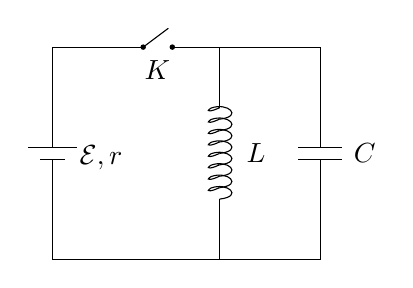
\begin{tikzpicture}[>=stealth]

\draw (0,0)--(3.4,0)--(3.4,1.27) (3.4,1.43)--(3.4,2.7)--(1.52,2.7) (1.15,2.7)--(0,2.7)--(0,1.43) (0,1.27)--(0,0)
(-.31,1.43)--(.31,1.43) (-.16,1.27)--(.16,1.27) (3.12,1.27)--(3.68,1.27) (3.12,1.43)--(3.68,1.43);
\draw(1.15,2.7)--(1.47,2.94);\fill (1.15,2.7)circle(.035) (1.52,2.7)circle(.035);
\node[below]at(1.33,2.65){$K$};\node[right]at(.22,1.30){$\mathcal E,r$};\node[right]at(3.7,1.35){$C$};
\draw (2.12,0)--(2.12,.77) (2.12,1.93)--(2.12,2.7);
\foreach \y in {.77,.915,1.06,1.205,1.35,1.495,1.64,1.785}{
 \begin{scope}[shift={(2.12,\y)}]\draw(0,0)..controls(.31,.035)and(.10,.22)..(-.11,.14)..controls(-.2,.08)and(-.08,.105)..(0,.145);\end{scope}}
\node[right]at(2.34,1.35){$L$};
\end{tikzpicture}\end{center}
В электрической цепи, показанной на рисунке, ключ К длительное время замкнут, $\mathcal E = 3\,\text{В},$ r = $2\,\text{Ом}$, L = $1$ мГн, С = $50$ мкФ. В момент t = $0$ ключ К размыкают. Каково напряжение U на конденсаторе в момент, когда в ходе возникших в контуре электромагнитных колебаний сила тока в контуре I = $1\,\text{А}$? Сопротивлением проводов и активным сопротивлением катушки индуктивности пренебречь.
}{
\smallskip\noindent\textbf{Решение}\par
Пока ключ замкнут через катушку течет постоянный ток $I_0,$ определяемый сопротивлением источника: $I_0 = \frac{\mathcal E}{r} .$ Поскольку активное сопротивление катушки, по условию, равно нулю, на катушке не падает напряжение, а значит, нулевое напряжение приложено к конденсатору. Таким образом, до размыкания ключа конденсатор разряжен. Начальная энергия электромагнитного поля в катушке $\frac{LI_0 ^2}{2} .$
После размыкания ключа начинаются электромагнитные колебания, и вся энергия, запасенная в катушке, будет перетекать из катушки в конденсатор и обратно. Энергия конденсатора равна $\frac{CU ^2}{2} .$ Через некоторое время энергия катушки уменьшится, а энергия конденсатора увеличится, причем сумма этих энергий будет равна начальной энергии катушки:

\[\frac{LI_0 ^2}{2} = \frac{LI ^2}{2} + \frac{CU ^2}{2} .\]

Откуда:

\[U = \sqrt{\frac{L ( I_0 ^2 - I ^2 )}{C}} = \sqrt{\frac{10^{-3} \,\text{Гн} \cdot \bigl( ( \frac{3\,\text{В}}{2\,\text{Ом}} ) ^2 - ( 1\,\text{А} ) ^2 \bigr)}{50 \cdot 10 ^{ - 6 } \,\text{Ф}}} = 5\,\text{В}.\]

Ответ: $5\,\text{В}$.
}

% Source 32270: https://phys-ege.sdamgia.ru/problem?id=32270
\BankTask{32270}{
В колебательном контуре, активное сопротивление которого равно нулю, происходят свободные электромагнитные колебания с периодом T  =  $50{,}24\,\text{мкс}$ и максимальным напряжением на конденсаторе $U_{max}$. Зависимость энергии электрического поля конденсатора от разности потенциалов между его обкладками в пределах от $0$ до $U_{max}$ приведена на графике. Определите максимальное значение силы тока в контуре.

\begin{center}\begin{tikzpicture}[>=stealth,line width=.65pt]\draw[step=.4,gray!50] (0,0)grid(4,4);\draw[->](0,0)--(5.15,0)node[below]{$U$, В};\draw[->](0,0)--(0,4.65)node[left]{$E_{\text{эл}}$, мДж};\node[below left]at(0,0){$0$};\node[left]at(0,2){$0{,}5$};\node[left]at(0,4){$1{,}0$};\node[below]at(2,0){$100$};\node[below]at(4,0){$200$};\draw[orange!80!black,domain=0:4,samples=55]plot(\x,{.2*\x*\x});\fill[orange!80!black](4,3.2)circle(.045);\end{tikzpicture}\end{center}
}{
\smallskip\noindent\textbf{Решение}\par
$1$.  По закону сохранения энергии при отсутствии активного сопротивления в колебательном контуре максимальная энергия заряженного конденсатора равна максимальной энергии магнитного поля катушки с током $W_p=W_{\,\text{м}}.$
При этом максимальная энергия катушки с током равна $W_{\,\text{м}}= \frac{LI ^2 _{\max}}{2} .$
$2$.  В условии задачи известен период колебаний. Период колебаний в колебательном контуре $T=2 \pi \sqrt{LC} .$
$3$.  Максимальная энергия заряженного конденсатора равна $W_{\,\text{р}}= \frac{CU_{\max} ^2}{2} .$
Тогда выражаем:

$C= \frac{2W_{\,\text{р}}}{U_{\max} ^2} ;$
$L= \frac{T ^2}{4 \pi ^2 C} ;$
$I_{\max}= \sqrt{\frac{2W_{\,\text{м}}}{L}} = \frac{4 \pi W_p}{TU_{\max}} .$

Из графика находим, что максимальное значение энергии электрического поля конденсатора $W_p=0{,}8 \cdot 10 ^{ - 3 } \,\text{Дж},$ максимальное напряжение на обкладках конденсатора $U_{\max}=200\,\text{В}.$ При подстановке значений в формулу получаем:

\[I_{\max}= \frac{4 \cdot 3{,}14 \cdot 0{,}8 \cdot 10 ^{ - 3 }}{50{,}24 \cdot 10 ^{ - 6 } \cdot 200} =1\,\text{А}.\]

Ответ: $1\,\text{А}$.
}

% Source 42802: https://phys-ege.sdamgia.ru/problem?id=42802
\BankTask{42802}{
\begin{center}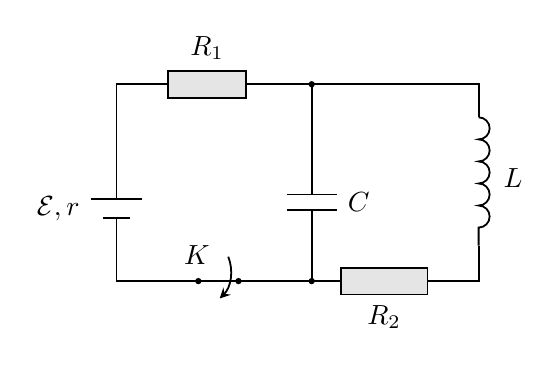
\begin{tikzpicture}[>=stealth,line width=.65pt]\draw (0,1.04)--(0,2.5)--(.65,2.5) (1.65,2.5)--(4.6,2.5)--(4.6,2.08) (4.6,.45)--(4.6,0)--(3.95,0) (2.85,0)--(1.55,0) (1.04,0)--(0,0)--(0,.8);\draw (2.48,2.5)--(2.48,1.1) (2.48,.9)--(2.48,0);\draw (-.32,1.04)--(.32,1.04) (-.17,.8)--(.17,.8) (2.16,1.1)--(2.8,1.1) (2.16,.9)--(2.8,.9);\draw[fill=gray!20](.65,2.33)rectangle(1.65,2.67) (2.85,-.17)rectangle(3.95,.17);\draw (4.6,2.08) arc(90:-90:.14) arc(90:-90:.14) arc(90:-90:.14) arc(90:-90:.14) arc(90:-90:.14) --(4.6,.45);\draw (1.04,0)--(1.55,0);\draw[->] (1.42,.31)arc(22:-45:.49);\foreach \p in {(1.04,0),(1.55,0),(2.48,0),(2.48,2.5)}{\fill \p circle(.04);}\node[left]at(-.34,.92){$\mathcal E,r$};\node[above]at(1.15,2.68){$R_1$};\node[below]at(3.4,-.18){$R_2$};\node[right]at(2.81,1){$C$};\node[right]at(4.79,1.31){$L$};\node[above]at(1.02,.08){$K$};\end{tikzpicture}\end{center}

Электрическая цепь состоит из источника питания с ЭДС $\mathcal{E} = 10\,\text{В}$ и внутренним сопротивлением $r = 1\,\text{Ом},$ двух резисторов с сопротивлениями $R_1 = 5\,\text{Ом}$ и $R_2 = 4\,\text{Ом},$ конденсатора электроёмкостью $C = 80\,\text{мкФ},$ катушки с индуктивностью $L = 200\,\text{мкГн}$ и замкнутого ключа К. Схема этой цепи показана на рисунке. Пренебрегая сопротивлением катушки, определите, какое количество теплоты Q выделится в резисторe $R_2$ в течение длительного времени после размыкания ключа К?
}{
\smallskip\noindent\textbf{Решение}\par
$1$.  До размыкания ключа через катушку течёт постоянный ток, сила которого, по закону Ома для замкнутой цепи, равна 

\[I = \frac{\mathcal{E}}{r + R_1 + R_2} .\]
 При этом напряжение на конденсаторе постоянно и равно падению напряжения на резисторе $R_2,$ поскольку конденсатор и ветвь цепи, содержащая последовательно соединённые резистор $R_2$ и идеальную катушку, соединены параллельно. Поэтому напряжение на конденсаторе равно $U_C = IR_2.$
$2$.  В замкнутом участке цепи, содержащем конденсатор, катушку и резистор $R_2,$ после размыкания ключа возникнут затухающие электромагнитные колебания. Спустя достаточно большое время они прекратятся. В процессе этих колебаний в резисторе $R_2,$ в соответствии с законом Джоуля-Ленца, будет выделяться количество теплоты.
$3$.  Из закона сохранения энергии, примененного для электрической цепи, следует, что к моменту полного затухания указанных колебаний выделившееся в резисторе $R_2$ количество теплоты Q будет равно сумме энергии, запасенной на момент размыкания ключа К в конденсаторе  $W_C= \frac{CU ^2 _C}{2} ,$ и энергии, запасённой в катушке  $W_L= \frac{LI ^2}{2} .$
$4$.  Подставляя в записанные формулы выражения для $U_{C}$ и I, с учётом численных значений физических величин, получим:

$Q=W_C + W_L= \frac{CU ^2 _C}{2} + \frac{LI ^2}{2} = \frac{CR ^2 _2 I ^2}{2} + \frac{LI ^2}{2} = \frac{I ^2 ( CR ^2 _2 + L )}{2} =$

$= \frac{\mathcal{E} ^2 ( CR ^2 _2 + L )}{2 ( r + R_1 + R_2 ) ^2} = \frac{10 ^2 \cdot ( 80 \cdot 10 ^{ - 6 } \cdot 4 ^2 + 200 \cdot 10 ^{ - 6 } )}{2 \cdot ( 1 + 5 + 4 ) ^2} =0{,}74\,\text{мДж}.$

Ответ: $Q= \frac{\mathcal{E} ^2 ( CR ^2 _2 + L )}{2 ( r + R_1 + R_2 ) ^2} =0{,}74\,\text{мДж}.$
}

\end{document}
